\documentclass[10pt,a4paper]{article}

\usepackage[utf8]{inputenc}
\usepackage[T1]{fontenc}
\usepackage[brazil]{babel}
\usepackage{lmodern}
\usepackage{geometry}
\geometry{
	top=1.2cm,
	bottom=1.3cm,
	left=1.5cm,
	right=1.5cm
}

\usepackage{xcolor}
% Paleta Institucional
\definecolor{bisnavy}{RGB}{14, 30, 54}
\definecolor{bisblue}{RGB}{28, 64, 105}
\definecolor{bistile}{RGB}{60, 100, 145}
\definecolor{bisterra}{RGB}{192, 75, 55}
\definecolor{bisgold}{RGB}{220, 150, 60}
\definecolor{bislight}{RGB}{240, 244, 250}
\definecolor{secondary}{RGB}{90, 100, 110}
\definecolor{rulecolor}{RGB}{215, 220, 225}
\definecolor{boxbg}{RGB}{248, 250, 252}

% Cores do Quote e Resumo Executivo
\definecolor{corFundoQuote}{RGB}{244, 247, 253}
\definecolor{corBarraQuote}{RGB}{28, 64, 105}
\definecolor{corAzulExecutivo}{RGB}{248, 251, 255}
\definecolor{corBordaExecutivo}{RGB}{215, 228, 245}

\usepackage{tikz}
\usetikzlibrary{shapes,positioning,calc}

\usepackage{graphicx}
\usepackage{booktabs}
\usepackage{enumitem}
\usepackage{caption}
\captionsetup{
	position=top,
	skip=3pt,
	labelfont={bf,footnotesize,color=bisnavy},
	textfont={footnotesize,color=bisnavy}
}

\usepackage{tcolorbox}
\tcbuselibrary{skins,breakable}

\usepackage{siunitx}
\sisetup{output-decimal-marker={,}}

\usepackage{hyperref}
\hypersetup{
	colorlinks=true,
	linkcolor=bisblue,
	urlcolor=bisblue,
	citecolor=bisblue
}

\tcbset{
	quotebox/.style={
		enhanced,
		colback=corFundoQuote,
		boxrule=0pt,
		frame hidden,
		borderline west={2.5pt}{0pt}{corBarraQuote},
		arc=0pt,
		left=10pt,
		right=10pt,
		top=6pt,
		bottom=6pt
	},
	resumobox/.style={
		colback=corAzulExecutivo,
		colframe=corBordaExecutivo,
		boxrule=0.5pt,
		arc=2.5pt,
		left=8pt,
		right=8pt,
		top=5pt,
		bottom=5pt
	},
	notabox/.style={
		colback=white,
		colframe=rulecolor,
		boxrule=0.6pt,
		arc=2pt,
		left=8pt,
		right=8pt,
		top=5pt,
		bottom=5pt
	},
	downloadbox/.style={
		colback=white,
		colframe=bistile!60,
		boxrule=0.6pt,
		arc=2pt,
		left=8pt,
		right=8pt,
		top=5pt,
		bottom=5pt
	}
}

\setlength{\parindent}{0pt}
\setlength{\parskip}{3.5pt}

% Comando único de cabeçalho
\newcommand{\cabecalhopadrao}{
	\noindent
	{\large \bfseries \color{bisnavy} Monitor da Inflação Alimentar}
	\vspace{3pt}
	\noindent
	{\footnotesize \color{secondary} Itaiguara de Oliveira Bezerra \quad\textbar\quad Economista Sênior e de Dados \quad\textbar\quad {\bfseries\color{bisblue}Por Estrato de Renda -- Setembro de 2026}}
	\vspace{1.5pt}
	\noindent
	{\footnotesize \color{secondary} \texttt{itaiguara-bezerra.github.io}}
	\vspace{0.10cm}
	{\color{rulecolor}\hrule height 0.6pt}
	\vspace{0.20cm}
}

\begin{document}
	
	% ==============================================================================
	% CAPA EDITORIAL (NÃO CONTADA NA NUMERAÇÃO DE PÁGINAS)
	% ==============================================================================
	\begin{titlepage}
		\newgeometry{top=0cm, bottom=0cm, left=0cm, right=0cm}
		\noindent
		\begin{tikzpicture}[x=1cm, y=1cm]
			\path (0,0) rectangle (21, 29.7);
			
			\fill[bisnavy] (0, 29.7) -- (21, 29.7) -- (21, 16.5) -- (0, 12.0) -- cycle;
			\fill[bisblue] (0, 12.0) -- (21, 16.5) -- (21, 14.8) -- (0, 10.3) -- cycle;
			\fill[bistile] (0, 10.3) -- (21, 14.8) -- (21, 13.8) -- (0, 9.3) -- cycle;
			\fill[bisterra] (0, 9.3) -- (21, 13.8) -- (21, 12.8) -- (0, 8.3) -- cycle;
			\fill[bisgold] (0, 8.3) -- (21, 12.8) -- (21, 12.3) -- (0, 7.8) -- cycle;
			
			\fill[bislight] (0, 2.2) -- (21, 2.2) -- (21, 11.0) -- (0, 6.5) -- cycle;
			\fill[bistile, opacity=0.15] (5, 2.2) -- (21, 9.5) -- (21, 2.2) -- cycle;
			\fill[bisnavy, opacity=0.08] (0, 2.2) -- (14, 2.2) -- (0, 7.0) -- cycle;
			
			\fill[bisnavy] (0, 0) rectangle (21, 2.2);
			\fill[bisterra] (0, 2.2) rectangle (21, 2.4);
			
			\draw[white, opacity=0.3, line width=1.2pt] (1.8, 17.0) -- (19.2, 21.0);
			\draw[bisgold, opacity=0.6, line width=0.8pt] (1.8, 16.5) -- (19.2, 20.5);
			
			\node[anchor=north west, text=white, opacity=0.80, font=\scriptsize\sffamily\bfseries] 
			at (1.8, 28.0) {RELATÓRIO DE MONITORAMENTO MACROECONÔMICO};
			
			\node[anchor=north west, text=white, font=\huge\sffamily\bfseries, text width=17.5cm, align=left] 
			at (1.8, 26.5) {Monitor da Inflação Alimentar};
			
			\node[anchor=north west, text=bisgold, font=\Large\sffamily\bfseries] 
			at (1.8, 23.2) {Por Estrato de Renda -- Setembro de 2026};
			
			\node[anchor=north, text=white, font=\Large\sffamily\itshape, text width=17.5cm, align=center] 
			at (10.5, 21.4) {A dinâmica dos preços alimentares nos diferentes estratos de renda familiar};
			
			\node[anchor=south east, align=right] at (19.2, 3.2) {
				\color{bisnavy}\bfseries\large Itaiguara de Oliveira Bezerra\\[3pt]
				\color{secondary}\footnotesize Economista Sênior e de Dados\\[2pt]
				\color{secondary}\footnotesize Pesquisador Independente\\[2pt]
				\color{bistile}\footnotesize \texttt{itaiguara@terra.com.br}\\[2pt]
				\color{bisnavy}\footnotesize \texttt{itaiguara-bezerra.github.io}\\[5pt]
				\color{black}\scriptsize\bfseries Divulgado em 09 de outubro de 2026.
			};
			
			\node[anchor=west, text=white, opacity=0.85, font=\scriptsize\sffamily] 
			at (1.8, 1.1) {Pesquisa Econômica Independente \quad\textbar\quad Metodologia POF / IBGE};
			
			\node[anchor=east, text=white, font=\scriptsize\sffamily\bfseries] 
			at (19.2, 1.1) {Série Histórica e Monitoramento Mensal};
		\end{tikzpicture}
	\end{titlepage}
	\restoregeometry
	
	% ==============================================================================
	% PÁGINA 1: INDICADORES, PANORAMA, FIGURA 1 E TABELA 1
	% ==============================================================================
	\cabecalhopadrao
	
	\noindent
	\begin{minipage}[t]{0.24\textwidth}
		\centering
		{\footnotesize \bfseries IPCA GERAL}\\[1.5pt]
		{\large \bfseries \color{bisterra} +0,82\%}\\[1pt]
		{\scriptsize Variação mensal}
	\end{minipage}
	\hfill
	\begin{minipage}[t]{0.24\textwidth}
		\centering
		{\footnotesize \bfseries IPCA -- DOMICÍLIO}\\[1.5pt]
		{\large \bfseries \color{bisterra} +0,96\%}\\[1pt]
		{\scriptsize Variação mensal}
	\end{minipage}
	\hfill
	\begin{minipage}[t]{0.24\textwidth}
		\centering
		{\footnotesize \bfseries RENDA MUITO BAIXA}\\[1.5pt]
		{\large \bfseries \color{bisterra} +0,76\%}\\[1pt]
		{\scriptsize Menor rendimento}
	\end{minipage}
	\hfill
	\begin{minipage}[t]{0.24\textwidth}
		\centering
		{\footnotesize \bfseries RENDA ALTA}\\[1.5pt]
		{\large \bfseries \color{bisterra} +0,96\%}\\[1pt]
		{\scriptsize Maior rendimento}
	\end{minipage}
	
	\vspace{0.15cm}
	{\color{rulecolor}\hrule height 0.6pt}
	\vspace{0.15cm}
	
	\begin{tcolorbox}[quotebox]
		\small\itshape
		``Em setembro, a inflação da alimentação no domicílio foi positiva em todos os estratos de renda, mas apresentou diferenças de intensidade. A variação foi de 0,76\% na Renda Muito Baixa e de 0,96\% na Renda Alta, enquanto a Renda Média registrou a maior taxa mensal, de 1,09\%, acima do IPCA Geral e do IPCA de Alimentação no Domicílio.''
		\vspace{3pt}
		\par\raggedleft\normalfont\footnotesize --- Itaiguara Bezerra, Economista Sênior e de Dados
	\end{tcolorbox}
	
	\vspace{0.10cm}
	
	\begin{tcolorbox}[resumobox]
		\noindent {\bfseries\normalsize \color{bisnavy} Resumo Executivo:}
		\begin{itemize}[leftmargin=12pt, itemsep=2pt, topsep=2pt, parsep=0pt]
			
			\item {\small Diferenças de intensidade na inflação alimentar em Setembro de 2026: a Renda Muito Baixa registrou variação de +0,76\%, enquanto a Renda Alta anotou +0,96\% (diferença de 0,20 p.p. entre os extremos).}
			
			\item {\small O IPCA de Alimentação no Domicílio, apurado pelo IBGE, registrou alta de +0,96\%, igual à estimada para o estrato de Renda Alta.}
			
			\item {\small A contribuição negativa de Proteínas Animais atenuou a inflação, sobretudo nos estratos de Renda Média-Alta (-0,11 p.p.) e Renda Alta (-0,07 p.p.).}
			
			\item {\small Frutas e Hortaliças foi o principal vetor de alta em todos os estratos, com contribuição de +0,67 p.p. na Renda Muito Baixa e de +1,09 p.p. na Renda Média.}
			
		\end{itemize}
	\end{tcolorbox}
	
	\vspace{0.12cm}
	
	\noindent {\large \bfseries \color{bisnavy} Panorama do Mês e Trajetória Recente}
	
	\vspace{0.06cm}
	
	{\small Os dados de Setembro de 2026 mostram a retomada das altas nos preços da alimentação no domicílio na maioria dos estratos e a manutenção de variações positivas em todas as faixas de renda. Conforme ilustra o painel à direita, a Renda Média registrou a maior inflação mensal (1,09\%), seguida pela Renda Alta (0,96\%) e pela Renda Muito Baixa (0,76\%). A trajetória semestral, apresentada no gráfico à esquerda, evidencia a recuperação das taxas após as quedas observadas em julho.}
	
	\vspace{0.06cm}
	
	\begin{figure}[h!]
		\centering
		\caption{Trajetória semestral e variação no mês: Estratos de Renda vs. IPCA Alimentação no Domicílio.}
		\vspace{2pt}
		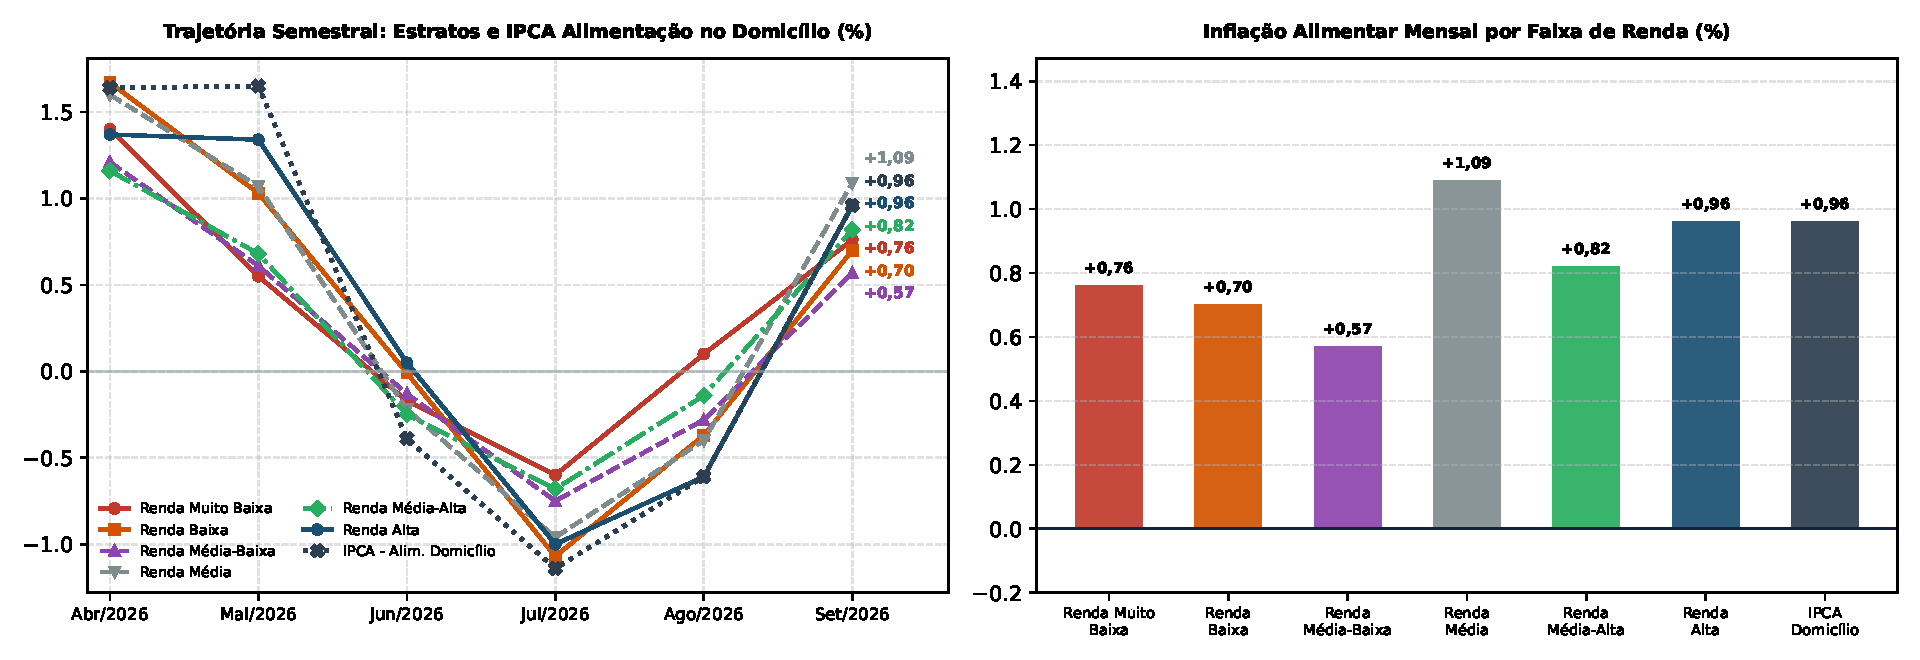
\includegraphics[width=\textwidth]{painel_1x2_trajetoria_barras.pdf}
		\vspace{2pt}
		\noindent\raggedright
		{\tiny \color{secondary} Fonte: Elaboração do autor com base em dados da POF 2017--2018 e Tabela 7060 (SIDRA/IBGE).}
	\end{figure}
	
	\vspace{0.15cm}
	
	\begin{table}[h!]
		\centering
		\caption{Variação Mensal e Acumulada (\%)}
		\vspace{1pt}
		\footnotesize
		\begin{tabular*}{\textwidth}{@{\extracolsep{\fill}} l c c c c c @{}}
			\toprule
			& \multicolumn{3}{c}{\textbf{Variação Mensal}} & \multicolumn{2}{c}{\textbf{Variação Acumulada}} \\
			\cmidrule(lr){2-4} \cmidrule(lr){5-6}
			\textbf{Estrato / Indicador} & \textbf{Jul./26} & \textbf{Ago./26} & \textbf{Set./26} & \textbf{12 Meses} & \textbf{No Ano} \\
			\midrule
			IPCA Geral & 0,07 & -0,32 & 0,82 & 4,58 & 3,95 \\
			IPCA - Alim. Domicílio & -1,14 & -0,61 & 0,96 & 4,19 & 4,42 \\
			\midrule
			
			Renda Muito Baixa & -0,60 & 0,10 & 0,76 & 5,42 & 4,66 \\
			
			Renda Baixa & -1,07 & -0,37 & 0,70 & 6,25 & 5,49 \\
			
			Renda Média-Baixa & -0,75 & -0,28 & 0,57 & 5,10 & 4,22 \\
			
			Renda Média & -0,96 & -0,40 & 1,09 & 6,52 & 5,30 \\
			
			Renda Média-Alta & -0,68 & -0,14 & 0,82 & 5,24 & 4,46 \\
			
			Renda Alta & -1,00 & -0,61 & 0,96 & 5,93 & 5,29 \\
			
			\bottomrule
		\end{tabular*}
	\end{table}
	
	\clearpage
	
	% ==============================================================================
	% PÁGINA 2: TENDÊNCIA E DECOMPOSIÇÃO
	% ==============================================================================
	\cabecalhopadrao
	
	\noindent {\large \bfseries \color{bisnavy} Análise de Tendência e Suavização}
	
	\vspace{0.06cm}
	
	{\small A comparação entre a tendência anualizada e a medida suavizada (EWMA) permite avaliar se a inflação alimentar está ganhando ou perdendo intensidade entre as diferentes faixas de renda. Valores da tendência anualizada superiores ao EWMA sugerem aceleração recente dos preços, enquanto valores inferiores indicam arrefecimento das pressões inflacionárias.}
	
	\vspace{0.25cm}
	
	\begin{table}[h!]
		\centering
		\caption{Tendências da Inflação Alimentar (\% ao ano)}
		\vspace{1pt}
		\footnotesize
		\begin{minipage}{0.80\textwidth}
			\begin{tabular*}{\linewidth}{@{\extracolsep{\fill}} l c c @{}}
				\toprule
				& \multicolumn{2}{c}{\textbf{Taxas Anualizadas (\% ao ano)}} \\
				\cmidrule(lr){2-3}
				\textbf{Faixa de Renda} & \begin{tabular}{@{}c@{}}\textbf{\color{bisnavy}Tendência} \\ \textbf{\color{bisnavy}(com base no resultado do mês)}\end{tabular} & \textbf{Suavização} \\
				\midrule
				
				Renda Muito Baixa & +9,51 & +4,35 \\
				
				Renda Baixa & +8,73 & +4,20 \\
				
				Renda Média-Baixa & +7,06 & +3,39 \\
				
				Renda Média & +13,89 & +4,66 \\
				
				Renda Média-Alta & +10,30 & +3,97 \\
				
				Renda Alta & +12,15 & +4,28 \\
				
				\bottomrule
			\end{tabular*}
			\vspace{4pt}\par
			\noindent
			{\tiny \color{secondary} \textbf{Nota Metodológica:} O método de suavização utilizado é a Média Móvel Exponencialmente Ponderada (EWMA). Para maiores detalhes sobre a modelagem, a Nota Técnica encontra-se disponível para \textit{download} na seção de \textbf{Repositório Público} (pág. 4).\par}
		\end{minipage}
	\end{table}
	
	\vspace{0.4cm}
	
	\noindent {\large \bfseries \color{bisnavy} O que Explicou a Variação Mensal}
	
	\vspace{0.06cm}
	
	{\small A decomposição das contribuições mensais mostra que Frutas e Hortaliças exerceu pressão positiva sobre a inflação em todos os estratos de renda, com maior contribuição na Renda Média (+1,09 p.p.), seguida pela Renda Alta (+0,89 p.p.) e pela Renda Média-Alta (+0,87 p.p.). Em sentido contrário, Proteínas Animais contribuiu negativamente para a variação mensal, atenuando as taxas na Renda Média-Alta (-0,11 p.p.) e na Renda Alta (-0,07 p.p.).}
	
	\vspace{0.08cm}
	
	\begin{figure}[h!]
		\centering
		\caption{Contribuições dos grupos de produtos para a inflação mensal, por estrato de renda (p.p.)}
		\vspace{2pt}
		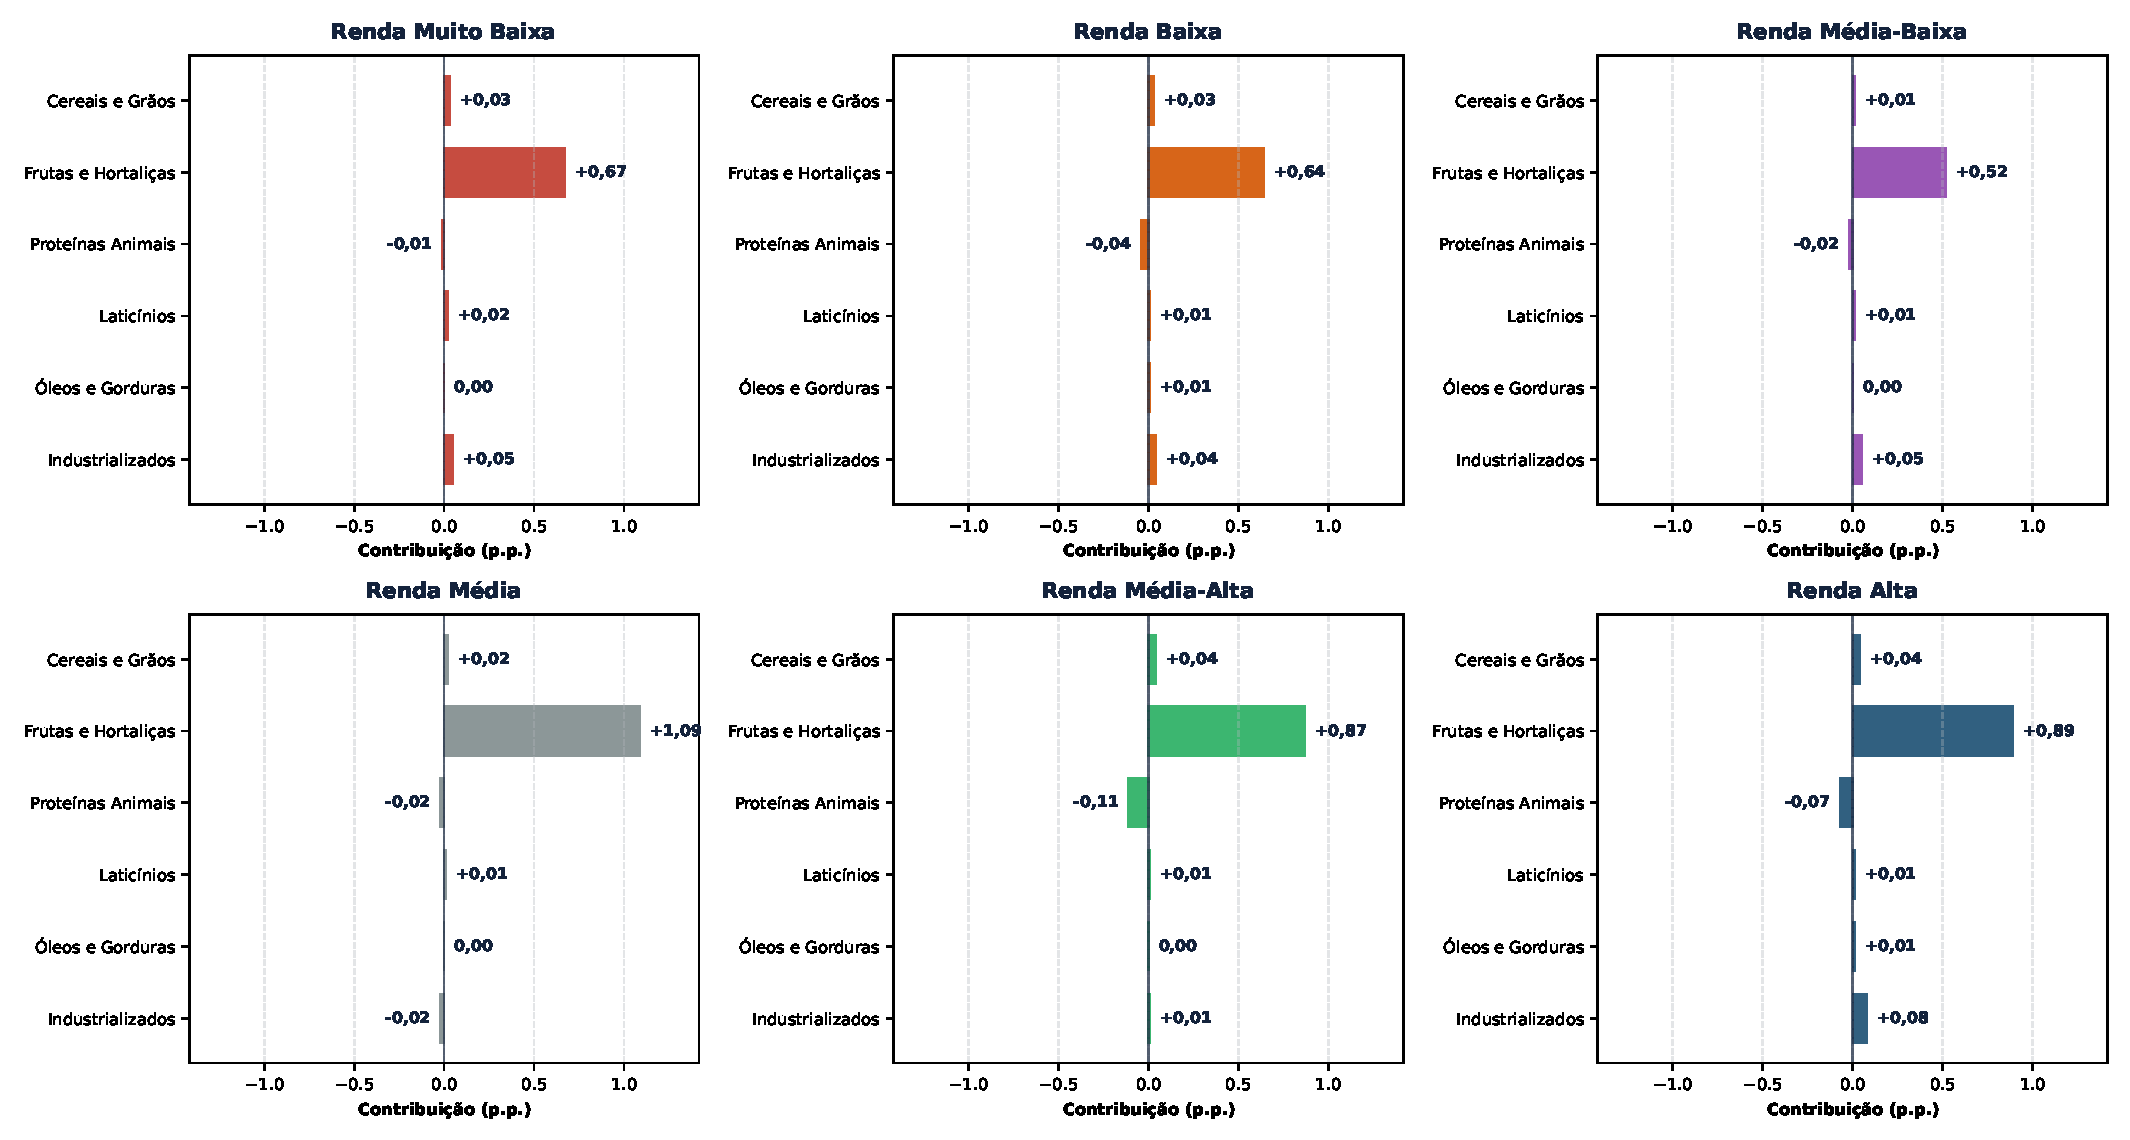
\includegraphics[width=\textwidth]{painel_contribuicao_6faixas.pdf}\par
		\vspace{4pt}
		\begin{flushleft}
			{\tiny \color{secondary} Fonte: Elaboração do autor com base em dados da POF 2017--2018 e Tabela 7060 (SIDRA/IBGE).\par}
		\end{flushleft}
	\end{figure}
	
	\clearpage
	
	% ==============================================================================
	% PÁGINA 3: TABELA 3 (SUBITENS)
	% ==============================================================================
	\cabecalhopadrao
	
	\noindent {\large \bfseries \color{bisnavy} Principais Contribuições Marginais de Subitens Alimentares por Estrato}
	\vspace{0.02cm}
	{\color{rulecolor}\hrule height 0.6pt}
	\vspace{0.06cm}
	
	{\small A tabela abaixo discrimina os cinco subitens que exerceram as maiores contribuições marginais positivas e negativas na formação da taxa mensal de cada estrato em Setembro de 2026.}
	
	\vspace{0.05cm}
	
	\begin{table}[h!]
		\centering
		\caption{Principais Contribuições Marginais de Subitens Alimentares por Estrato (Setembro de 2026)}
		\vspace{2pt}
		\footnotesize
		\renewcommand{\arraystretch}{1.15} % Aumenta o espaçamento vertical entre as linhas
		\setlength{\tabcolsep}{7pt} % Aumenta o respiro horizontal das colunas
		\begin{tabular*}{\textwidth}{@{\extracolsep{\fill}} c l c c | l c c @{}}
			\toprule
			& \multicolumn{3}{c}{\textbf{Maiores Altas (+) por Contribuição}} & \multicolumn{3}{c}{\textbf{Maiores Quedas (--) por Contribuição}} \\
			\cmidrule(lr){2-4} \cmidrule(lr){5-7}
			\textbf{\#} & \textbf{Alimento} & \textbf{Var. (\%)} & \textbf{Contrib. (p.p.)} & \textbf{Alimento} & \textbf{Var. (\%)} & \textbf{Contrib. (p.p.)} \\
			\midrule
			
			\multicolumn{7}{l}{\textbf{\color{bisnavy}Renda Muito Baixa}} \\
			\midrule
			
			1 & Limão & +46,42 & +0,3112 & Manga & -9,62 & -0,1047 \\
			
			2 & Abobrinha & +29,82 & +0,1754 & Melancia & -8,11 & -0,0860 \\
			
			3 & Tomate & +37,76 & +0,1193 & Pimentão & -10,95 & -0,0828 \\
			
			4 & Melão & +9,90 & +0,1009 & Peixe - dourada & -9,06 & -0,0585 \\
			
			5 & Couve-flor & +9,58 & +0,0899 & Cenoura & -6,41 & -0,0338 \\
			
			\midrule
			
			\multicolumn{7}{l}{\textbf{\color{bisnavy}Renda Baixa}} \\
			\midrule
			
			1 & Tomate & +37,76 & +0,1796 & Melancia & -8,11 & -0,0636 \\
			
			2 & Batata-inglesa & +24,07 & +0,1789 & Cenoura & -6,41 & -0,0634 \\
			
			3 & Abobrinha & +29,82 & +0,1538 & Morango & -6,04 & -0,0503 \\
			
			4 & Limão & +46,42 & +0,1230 & Banana - prata & -3,88 & -0,0375 \\
			
			5 & Melão & +9,90 & +0,0742 & Pimentão & -10,95 & -0,0325 \\
			
			\midrule
			
			\multicolumn{7}{l}{\textbf{\color{bisnavy}Renda Média-Baixa}} \\
			\midrule
			
			1 & Abobrinha & +29,82 & +0,2850 & Pimentão & -10,95 & -0,0668 \\
			
			2 & Limão & +46,42 & +0,2463 & Mamão & -6,59 & -0,0660 \\
			
			3 & Tomate & +37,76 & +0,1018 & Peixe - dourada & -9,06 & -0,0634 \\
			
			4 & Batata-inglesa & +24,07 & +0,0689 & Morango & -6,04 & -0,0571 \\
			
			5 & Cebola & +10,14 & +0,0635 & Cenoura & -6,41 & -0,0391 \\
			
			\midrule
			
			\multicolumn{7}{l}{\textbf{\color{bisnavy}Renda Média}} \\
			\midrule
			
			1 & Limão & +46,42 & +0,4279 & Melancia & -8,11 & -0,0767 \\
			
			2 & Tomate & +37,76 & +0,3936 & Morango & -6,04 & -0,0614 \\
			
			3 & Abobrinha & +29,82 & +0,1465 & Repolho & -6,06 & -0,0573 \\
			
			4 & Cebola & +10,14 & +0,1068 & Cenoura & -6,41 & -0,0511 \\
			
			5 & Batata-inglesa & +24,07 & +0,1020 & Peixe - dourada & -9,06 & -0,0480 \\
			
			\midrule
			
			\multicolumn{7}{l}{\textbf{\color{bisnavy}Renda Média-Alta}} \\
			\midrule
			
			1 & Limão & +46,42 & +0,3722 & Peixe - dourada & -9,06 & -0,0849 \\
			
			2 & Tomate & +37,76 & +0,1963 & Melancia & -8,11 & -0,0726 \\
			
			3 & Abobrinha & +29,82 & +0,1739 & Manga & -9,62 & -0,0685 \\
			
			4 & Batata-inglesa & +24,07 & +0,1638 & Pimentão & -10,95 & -0,0489 \\
			
			5 & Couve-flor & +9,58 & +0,0970 & Mamão & -6,59 & -0,0460 \\
			
			\midrule
			
			\multicolumn{7}{l}{\textbf{\color{bisnavy}Renda Alta}} \\
			\midrule
			
			1 & Abobrinha & +29,82 & +0,3105 & Melancia & -8,11 & -0,0902 \\
			
			2 & Tomate & +37,76 & +0,2776 & Peixe - dourada & -9,06 & -0,0776 \\
			
			3 & Batata-inglesa & +24,07 & +0,2649 & Pimentão & -10,95 & -0,0731 \\
			
			4 & Limão & +46,42 & +0,1630 & Morango & -6,04 & -0,0616 \\
			
			5 & Pepino & +6,99 & +0,0695 & Manga & -9,62 & -0,0549 \\
			
			\midrule
			
			\bottomrule
		\end{tabular*}
		\vspace{3pt}
		\noindent\raggedright
		{\tiny \color{secondary} Fonte: Elaboração do autor com base na POF 2017--2018 e Tabela 7060 (SIDRA/IBGE). Nota: A ordenação é dada estritamente pela contribuição em pontos percentuais. A recorrência dos mesmos itens entre estratos decorre de a variação de preço ser uniforme nacionalmente.}
	\end{table}
	
	\clearpage
	
	% ==============================================================================
	% PÁGINA 4: FAIXAS DE RENDA E REPOSITÓRIO PÚBLICO
	% ==============================================================================
	\cabecalhopadrao
	
	\noindent {\large \bfseries \color{bisnavy} Classificação Socioeconômica e Repositório Público}
	\vspace{0.02cm}
	{\color{rulecolor}\hrule height 0.6pt}
	\vspace{0.08cm}
	
	\noindent {\normalsize \bfseries \color{bisnavy} Estratificação Socioeconômica e Ponderação de Consumo}
	\vspace{0.06cm}
	
	{\small A classificação dos estratos adota a padronização oficial do Indicador Ipea de Inflação por Faixa de Renda, calibrada pela inflação acumulada e ancorada na POF 2017--2018.}
	
	\vspace{0.04cm}
	
	\begin{table}[h!]
		\centering
		\caption{Faixas de Renda Mensal Domiciliar}
		\vspace{2pt}
		\footnotesize
		\begin{tabular*}{\textwidth}{@{\extracolsep{\fill}} l c c @{}}
			\toprule
			\textbf{Faixa de Renda} & \textbf{Renda Domiciliar (jan./2009)} & \textbf{Renda Domiciliar (jan./2026)} \\
			\midrule
			
			1 -- Renda muito baixa & Menor que R\$ 900,00 & Menor que R\$ 2.299,82 \\
			
			2 -- Renda baixa & De R\$ 900,00 a R\$ 1.350,00 & De R\$ 2.299,82 a R\$ 3.449,73 \\
			
			3 -- Renda média-baixa & De R\$ 1.350,01 a R\$ 2.250,00 & De R\$ 3.449,74 a R\$ 5.749,55 \\
			
			4 -- Renda média & De R\$ 2.250,01 a R\$ 4.500,00 & De R\$ 5.749,56 a R\$ 11.499,11 \\
			
			5 -- Renda média-alta & De R\$ 4.500,01 a R\$ 9.000,00 & De R\$ 11.499,12 a R\$ 22.998,22 \\
			
			6 -- Renda alta & Maior que R\$ 9.000,00 & Maior que R\$ 22.998,22 \\
			
			\bottomrule
		\end{tabular*}
		\vspace{2pt}
		\noindent\raggedright
		{\tiny \color{secondary} Fonte: Elaboração do autor com base na Carta de Conjuntura, Dimac/Ipea.}
	\end{table}
	
	\vspace*{\fill}
	
	\noindent {\normalsize \bfseries \color{bisnavy} Acesso Direto à Base de Dados e Edições Anteriores}
	\vspace{0.06cm}
	
	{\small Para garantir transparência analítica e permitir auditoria independente, a série histórica completa cobrindo de Janeiro de 2020 a Setembro de 2026 --- acompanhada das matrizes de ponderação da POF 2017--2018, dos microdados dos subitens e da série de números-índice encadeados com base fixada em Janeiro de 2020 ($= 100{,}00$) --- encontra-se disponibilizada em repositório público:}
	
	\vspace{0.06cm}
	
	\begin{tcolorbox}[downloadbox]
		\centering
		{\bfseries \color{bisnavy} Repositório Institucional de Dados e Relatórios}\\[2pt]
		{\footnotesize \color{secondary} Série Histórica (Jan/2020 a Setembro de 2026)}\\[5pt]
		
		{\small
			\textbf{Edição Anterior (Agosto de 2026) (PDF):} \href{https://raw.githubusercontent.com/Itaiguara-Bezerra/itaiguara-bezerra.github.io/main/edicoes_anteriores/Monitor_Inflacao_Alimentar_anterior.pdf}{download direto}\\[4pt]
			\textbf{Nota Técnica Metodológica (PDF):} \href{https://raw.githubusercontent.com/Itaiguara-Bezerra/itaiguara-bezerra.github.io/main/dados/Nota_Tecnica_IPCA_Alimentacao_No_Domicilio_Por_Estrato_Socioeconomico_Versão_2.0.pdf}{download direto}\\[4pt]
			\textbf{Série de variações mensais (\%):} \href{https://raw.githubusercontent.com/Itaiguara-Bezerra/itaiguara-bezerra.github.io/main/dados/inflacao_mensal_ipca_renda_09_2026.xlsx}{.xlsx} \quad\textbar\quad \href{https://raw.githubusercontent.com/Itaiguara-Bezerra/itaiguara-bezerra.github.io/main/dados/inflacao_mensal_ipca_renda_09_2026.csv}{.csv} \quad\textbar\quad \href{https://raw.githubusercontent.com/Itaiguara-Bezerra/itaiguara-bezerra.github.io/main/dados/inflacao_mensal_ipca_renda_09_2026.parquet}{.parquet}\\[3pt]
			\textbf{Série de índices encadeados (Base 100 = Jan/2020):} \href{https://raw.githubusercontent.com/Itaiguara-Bezerra/itaiguara-bezerra.github.io/main/dados/indices_base100_ipca_renda_09_2026.xlsx}{.xlsx} \quad\textbar\quad \href{https://raw.githubusercontent.com/Itaiguara-Bezerra/itaiguara-bezerra.github.io/main/dados/indices_base100_ipca_renda_09_2026.csv}{.csv} \quad\textbar\quad \href{https://raw.githubusercontent.com/Itaiguara-Bezerra/itaiguara-bezerra.github.io/main/dados/indices_base100_ipca_renda_09_2026.parquet}{.parquet}
		}
	\end{tcolorbox}
	
	\vspace{0.10cm}
	
	\begin{tcolorbox}[notabox]
		{\bfseries \color{bisnavy} Nota de Isenção de Responsabilidade:}\\[2pt]
		{\footnotesize \color{secondary} As opiniões, análises e estimativas expressas neste relatório são de estrita e exclusiva responsabilidade do autor, não refletindo necessariamente a visão ou posicionamento oficial de quaisquer instituições com as quais mantenha vínculo profissional.}
	\end{tcolorbox}
	
	\vspace{0.08cm}
	
	\begin{tcolorbox}[notabox]
		{\bfseries \color{bisnavy} Como citar este documento:}\\[2pt]
		{\footnotesize \color{secondary} BEZERRA, Itaiguara de Oliveira. \textbf{Monitor da Inflação Alimentar: por Estrato de Renda}. Relatório de Acompanhamento Macroeconômico, Rio de Janeiro, Setembro de 2026. É permitida a reprodução total ou parcial das informações, tabelas e metodologias aqui contidas, desde que expressamente citada a fonte e atribuída a autoria. Reproduções para fins comerciais são proibidas.}
	\end{tcolorbox}
	
	\vspace{0.10cm}
	{\color{rulecolor}\hrule height 0.5pt}
	\vspace{2pt}
	{\tiny \color{secondary} Relatório técnico independente. Fontes dos dados brutos: IBGE (POF / SIDRA).}
	
\end{document}